\documentclass[aspectratio=169]{beamer} %% for 16:9 use this line
%%\documentclass{beamer} %% For 4:3 ratio use this line
\usepackage[utf8]{inputenc}
\usepackage[T1]{fontenc}
\usepackage{lipsum} 
\usepackage{bm}
\usepackage{hyperref}
\usepackage{graphicx}
\usepackage{animate}
\usepackage{multimedia}
\usepackage{amsmath}
\usepackage{subcaption}
\usepackage{tikz}
\usepackage{soul}
\usepackage{amssymb}% http://ctan.org/pkg/amssymb
\usepackage{pifont}% http://ctan.org/pkg/pifont
\newcommand{\cmark}{\ding{51}}%
\newcommand{\xmark}{\ding{55}}%
\captionsetup[figure]{font=footnotesize}
% import citation package
\usepackage[backend=biber, style=authoryear]{biblatex}
\addbibresource{../../conference/biblio.bib}
\AtBeginBibliography{\small}
\DeclareMathOperator*{\argmin}{\arg\!\min}
% footnote without number
\newcommand\blfootnote[1]{
\begingroup
\renewcommand\thefootnote{}\footnote{#1}
\addtocounter{footnote}{-1}
\endgroup
}

\usetheme{CEA2023}
\setlength{\columnsep}{0.05cm}
\title{Marius Duvillard - Réunion de suivi juin 2024}
\date[25-06-2024] %optional
{25 juin 2024}
\author[M. Duvillard] %optionam
{Marius Duvillard \inst{1} \inst{2} \texttt{(\small marius.duvillard\myat cea.fr)} \\
Olivier Le Maître \inst{2} \inst{3} \texttt{(\small olivier.le-maitre\myat polytechnique.edu)} \\
Michel Freyss \inst{1} \texttt{(\small michel.freyss \myat cea.fr)}\\
}

\institute[short-inst]{
 \inst{1} CEA DES/IRESNE/DEC/SESC Cadarache 
 \inst{2} Centre de Mathématiques Appliquées, Ecole Polytechnique 
 \inst{3} CNRS, Inria
}

% uncomment the following lines if you do not want dedicated outlines before
% each section
\AtBeginSection{}

% use your thanks-message in the last frame
\setvalue{\ThxMessage}{Thanks! Any questions?}
% Change the logo 
\titlegraphic{logos/LOGO_CEA_ORIGINAL.png}

% introduce another logo for a second author or affiliation
% secondlogo applies to the first page only
\setvalue{\secondlogo}{logos/Polytechnique_logo.pdf}

\begin{document}

% info: the plain removes the footline from the titlepage; noframenumbering
% neglects it from the total count of the slides
\begin{frame}[decorated] %Decorated bring the logo and corner
    \titlepage
\end{frame}

\begin{frame}[righttransition]{Outline} % or Table of Contents
    \tableofcontents
\end{frame}

\section{Derniers résultats}
\transition[1]{Derniers résultats}{Assimilation par alignement}

\begin{frame}{Correction de position}
    \vspace{-0.9cm}
    \begin{eqnarray*}
        u_i^f(x) &=& \sum_{p \in \mathcal P_i} \Gamma^f_p \phi_h(x - \textcolor{ceared}{x_p^f}), \quad u^a_i(x) = u_i^f(x) + \sum_{j=1}^{N_{\text{ens}}} F_{ij} u_j^f(x), \\
        u_i^a(x) &\approx& \sum_{p \in \mathcal P_i} \Gamma^f_p \phi_h(x - \textcolor{ceared}{A_i(x_p^f)}), \\
    \end{eqnarray*}
    \vspace{-0.7cm}

    \begin{columns}[t]
        \begin{column}{0.6\textwidth}
            $A_i$ est une transformation $x^a_{p} = A_i(x^f_{p})$. \\
            On choisit~\footnotemark[1] d'écrire $A(x)$ comme la solution de\\
            \begin{equation*}
                \begin{cases}
                    x'(\tau = 0) = x,                                           \\
                    \frac{d x'}{d \tau} = w_i (x'), \quad A_i(x) = x'(\tau = 1) \\
                \end{cases}
            \end{equation*}avec $w_i$ un champ de vitesse \textbf{à définir}
        \end{column}
        \begin{column}{0.4\textwidth}
            \vspace{-2cm}
            \begin{figure}
                \centering
                \only<1>{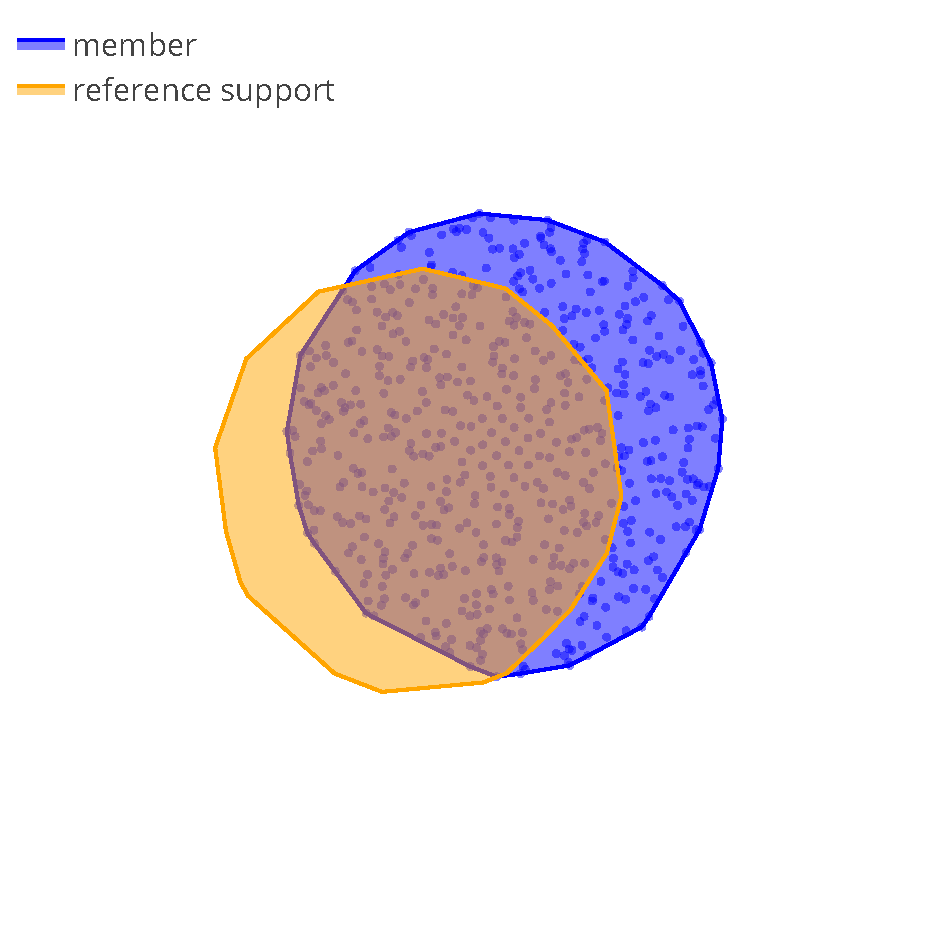
\includegraphics[width=0.8\textwidth]{../../conference/images/align_member_0.pdf}}
                \only<2>{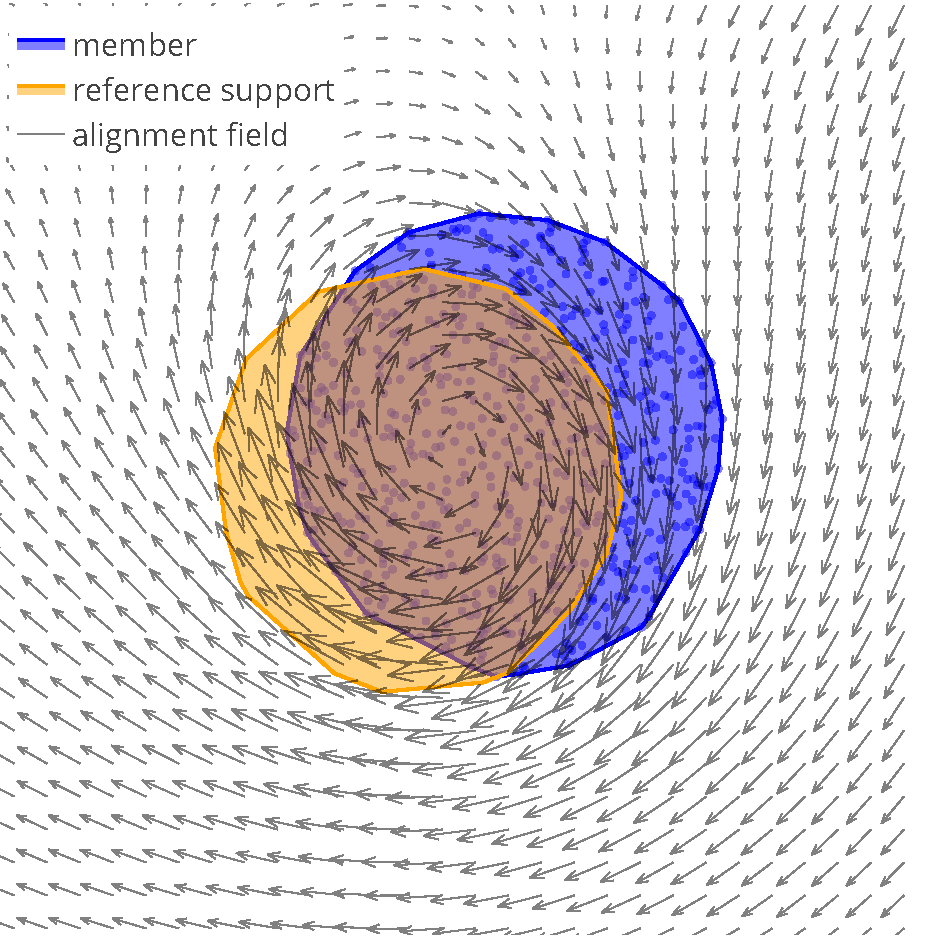
\includegraphics[width=0.8\textwidth]{../../conference/images/align_member_1.pdf}}
                \only<3>{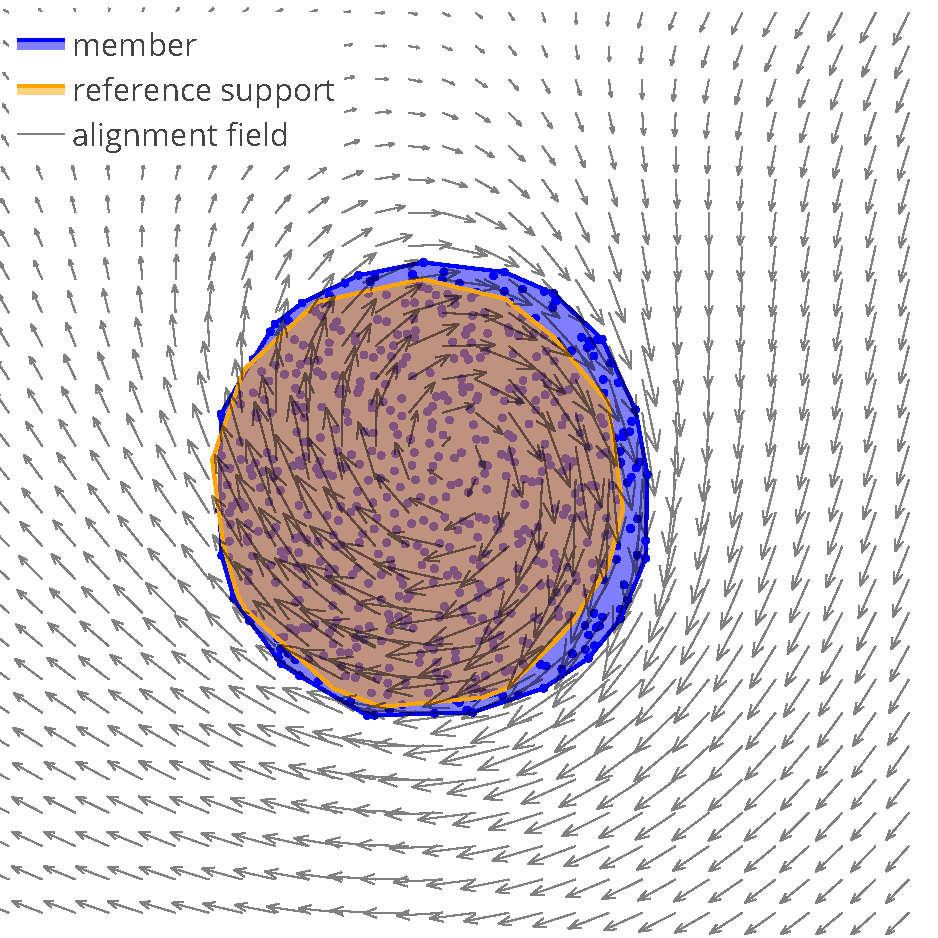
\includegraphics[width=0.8\textwidth]{../../conference/images/align_member_2_1.pdf}}
            \end{figure}
        \end{column}
    \end{columns}
    \vfill
    \footnotetext[1]{\tiny Other hypothesis have been made see~\cite{ravela_data_2007,rosenthal_displacement_2017}}
\end{frame}

\begin{frame}{Choix de $w_i$}
    Pour le membre $i$, on cherche à réduire l'écart entre les \textbf{prédictions} et les \textbf{observations}:
    \begin{equation*}
        w_i = \argmin_{w_i \in \mathcal V} \left\|y - \mathcal H(\mathcal{P}_i^f \mid w_i) \right\|^2_{R^{-1}} \visible<2->{\textcolor{ceared}{+ R(w)}}, \quad i = 1, \dots, N_{\text{ens}}
    \end{equation*}with $\mathcal V$ l'espace de recherche, $\mathcal H(\mathcal{P}_i^f \mid w_i)$ l'opérateur d'observation conditionné par $w_i$\\
    \vfill
    \visible<2->{\textcolor{ceared}{$R(w)$} est un terme de régularisation (éviter un mauvais conditionnement ou la non unicité)\\}
    \vfill
    \visible<2->{Problème défini sur un espace \textbf{infini}}
    \vfill
\end{frame}

\begin{frame}{Formulation d'ordre réduit}

    On cherche le champ d'alignement comme la combinaison linéaire des champs de vitesse des membres,\\
    find $\bm a_i \in \mathbb{R}^{N_{\text{ens}}}$ \\
    \begin{equation*}
        w_i = \sum_{j=1}^{N_{\text{ens}}} a_{i,j} v_j (x) = \sum_{j=1}^{N_{\text{ens}}} a_{i,j} \left(\sum_{p \in \mathcal P_j} \Gamma_p^f \vec{V}(x - x_p) + v_{j,BC} \right)
    \end{equation*}
    \vfill
    \visible<2->{$N_{\text{ens}}$ problèmes indépendants de dimension $N_{\text{ens}}$ \\
        \begin{equation*}
            \mathcal L_i (a) = \min_{a \in \mathbb{R}^{N_{\text{ens}}}} \left\|d - \mathcal H_a(\hat u^f_i; a) \right\|^2_{R^{-1}} + \lambda \|a\|_2^2, \quad i = 1, \dots, N_{\text{ens}}
        \end{equation*}
        Optimisés avec un optimiseur par descente de gradient (BFGS)}
    \vfill

\end{frame}

\begin{frame}{Problème des trois vortex(corps)}
    \vspace{-0.5cm}
    \begin{columns}[t]
        \begin{column}{0.45\textwidth}
            \begin{itemize}
                \item \scriptsize \textbf{Variables d'intérêt}: positions of vortex centers
                \item \scriptsize \textbf{Incertitude initiale}: centre des tourbillons, amplitude, taille de coeur,...
                \item \scriptsize \textbf{Trajectoires chaotiques}~\footnotemark[1]
                \item \scriptsize \textbf{observations}: Une grille de vitesse grossière et bruitée
            \end{itemize}
            \begin{figure}
                \centering
                \vspace{-0.25cm}
                % \only<2->{\caption*{\tiny Vortex normalized position error}}
                \includegraphics<3->[width=\textwidth]{../../conference/images/error_position_wo_assim.pdf}
            \end{figure}
            \vfill
        \end{column}
        \begin{column}{0.55\textwidth}
            \centering
            \begin{figure}[t]
                \centering
                \visible<2->{\tiny Trajectoire des centre de vortex après perturbation}
                \only<3->{%
                    \animategraphics[loop, autoplay, width=0.85\textwidth]{10}{../../conference/images/vortex_centers_disperse/vortex_centers_}{0}{36}%
                }
                \only<2>{%
                    \animategraphics[loop, autoplay, width=0.85\textwidth]{10}{../../conference/images/vortex_centers_ref/vortex_centers_}{0}{36}
                }
                \only<1>{%
                    \animategraphics[loop, autoplay, width=0.7\textwidth]{5}{../../conference/images/particles_ref/particles_ref_}{0}{20}
                }
            \end{figure}
        \end{column}
    \end{columns}
    \vspace{-0.5cm}

    \footnotetext[1]{\tiny \cite{aref_motion_1979}}
\end{frame}

\begin{frame}{Remesh-EnKF}
    \begin{columns}[t]
        \begin{column}{0.5\textwidth}
            \vspace{-0.5cm}
            \begin{figure}
                \centering
                \animategraphics[loop, autoplay, width=\textwidth]{10}{../../conference/images/vortex_centers_part_enkf/vortex_centers_}{0}{36}
            \end{figure}
        \end{column}
        \begin{column}{0.5\textwidth}
            \begin{figure}
                \centering
                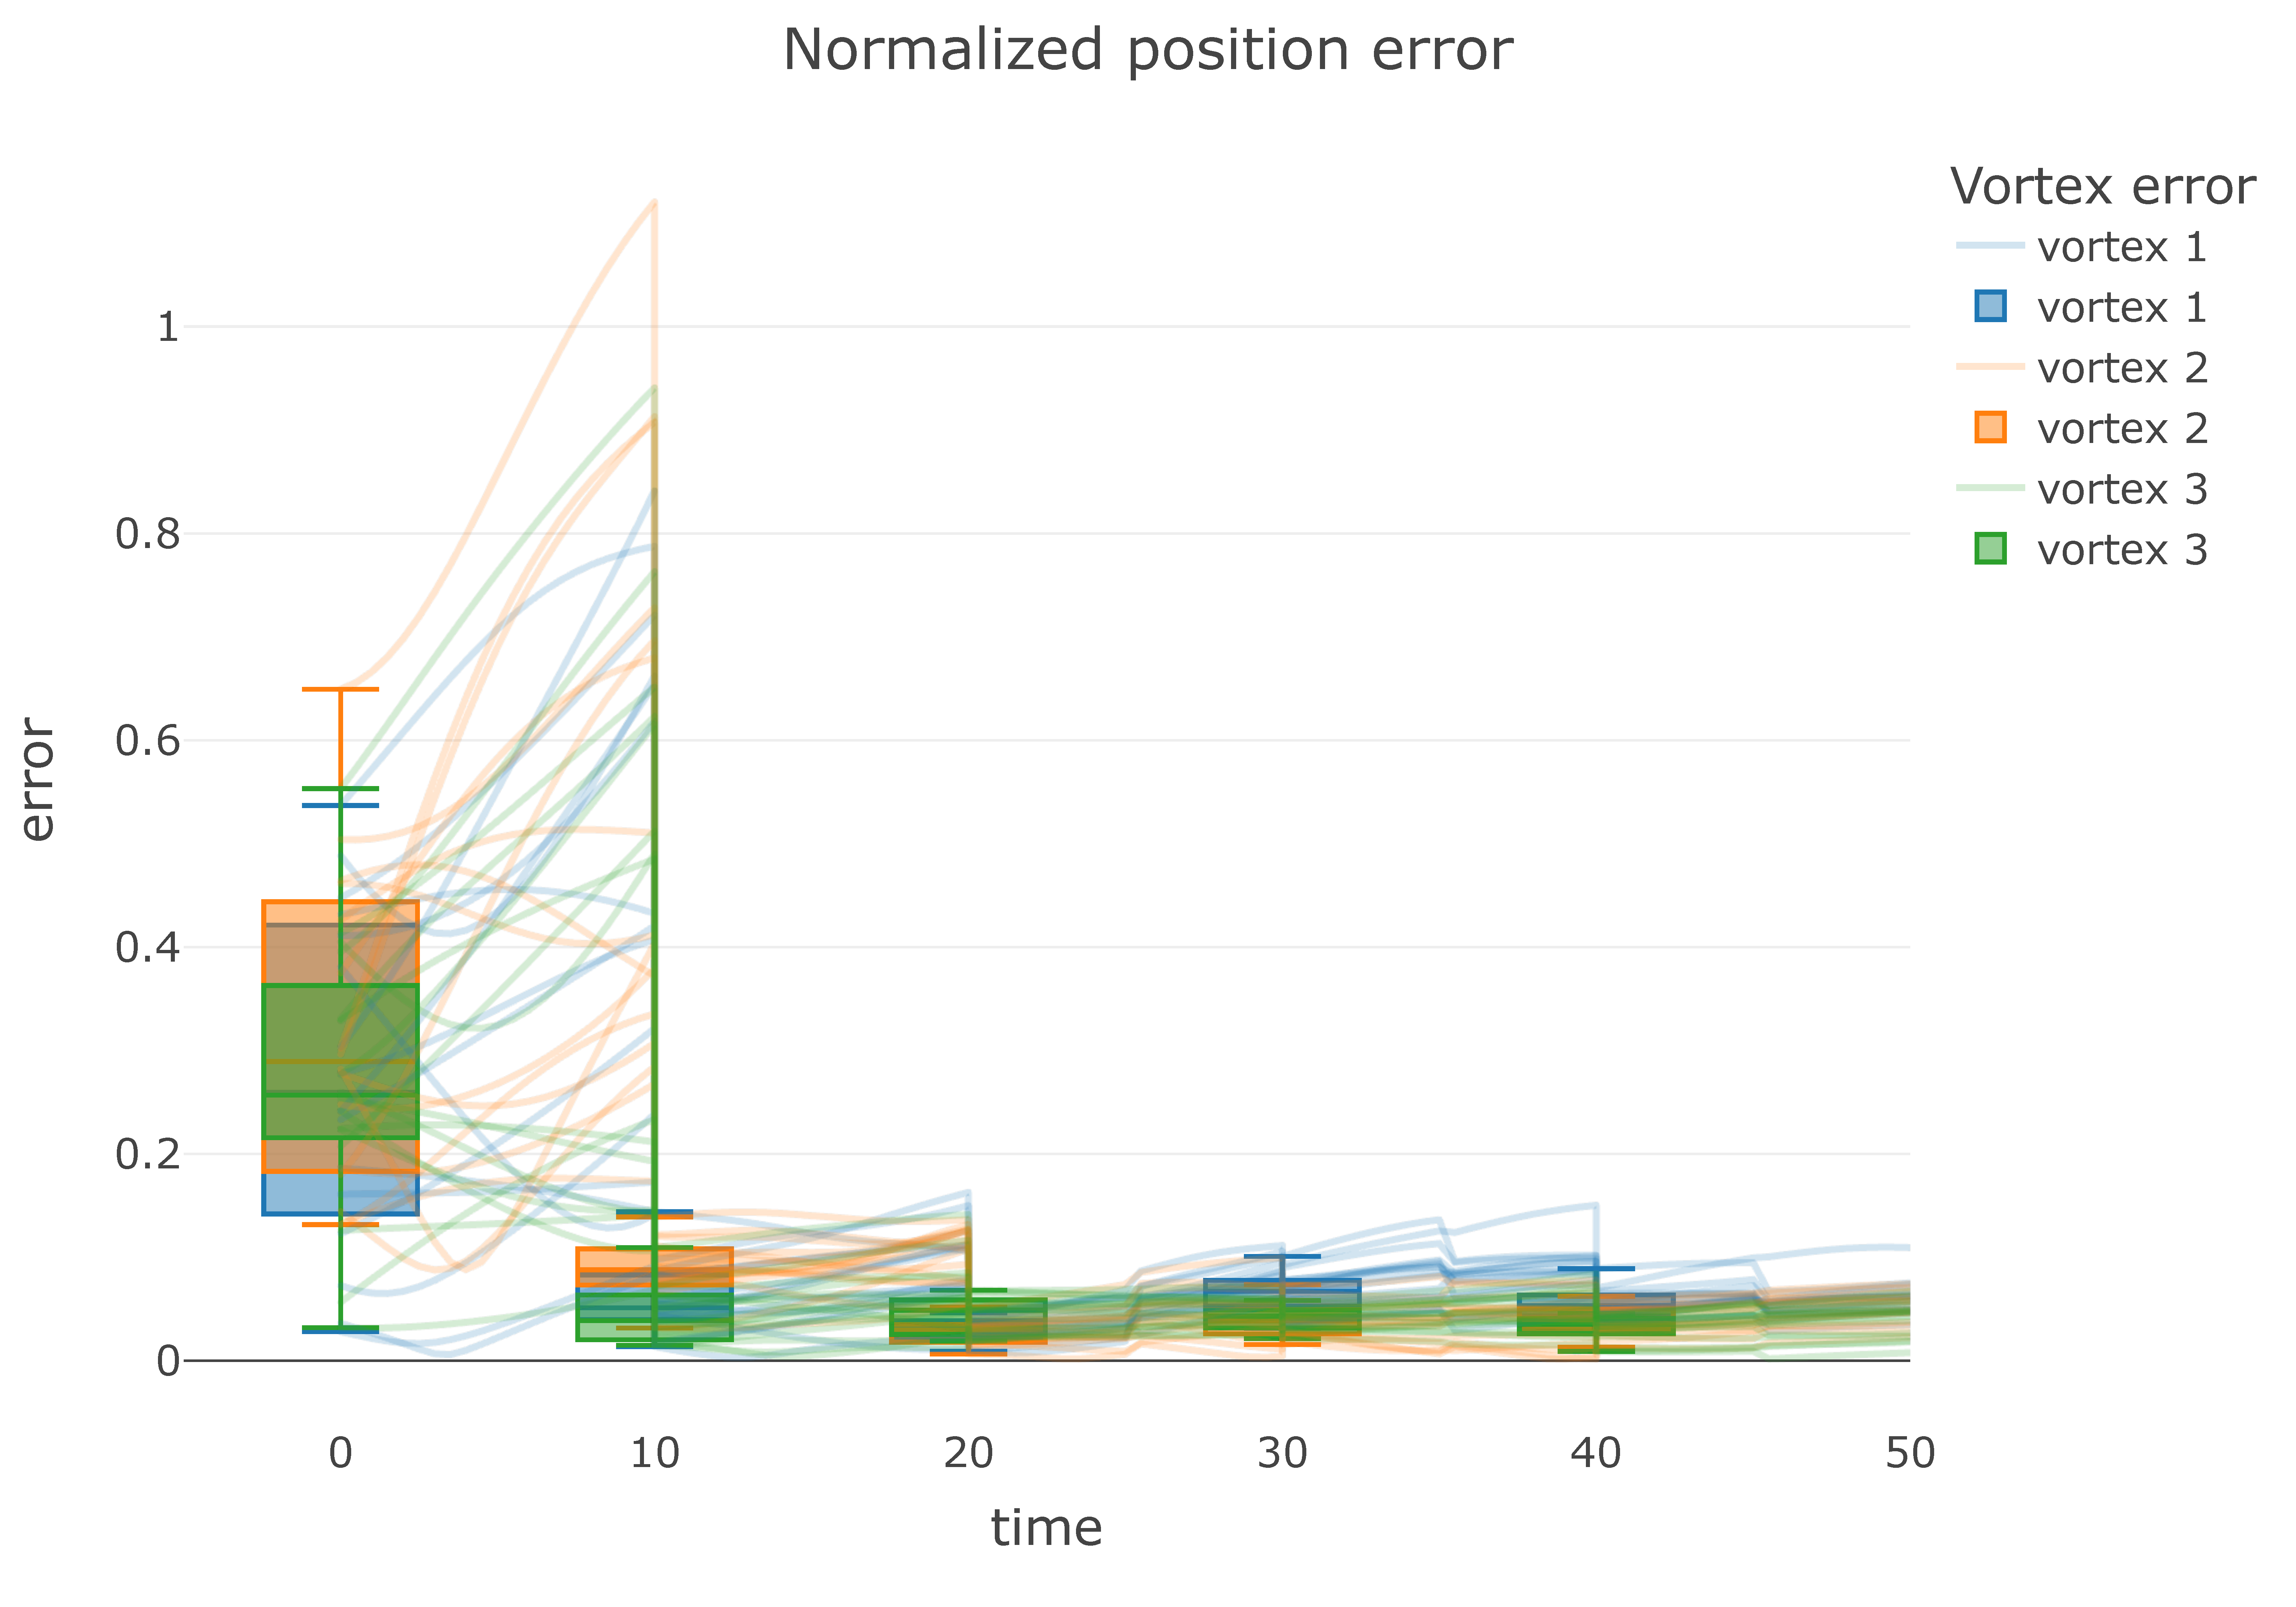
\includegraphics[width=\textwidth]{../../conference/images/remesh_enkf_error.pdf}
            \end{figure}
        \end{column}
    \end{columns}
\end{frame}

\begin{frame}{Part-EnKF}
    \begin{columns}[t]
        \begin{column}{0.5\textwidth}
            \vspace{-0.5cm}
            \begin{figure}
                \centering
                \animategraphics[loop, autoplay, width=\textwidth]{10}{../../conference/images/vortex_centers_part_enkf/vortex_centers_}{0}{36}
            \end{figure}
        \end{column}
        \begin{column}{0.5\textwidth}
            \begin{figure}
                \centering
                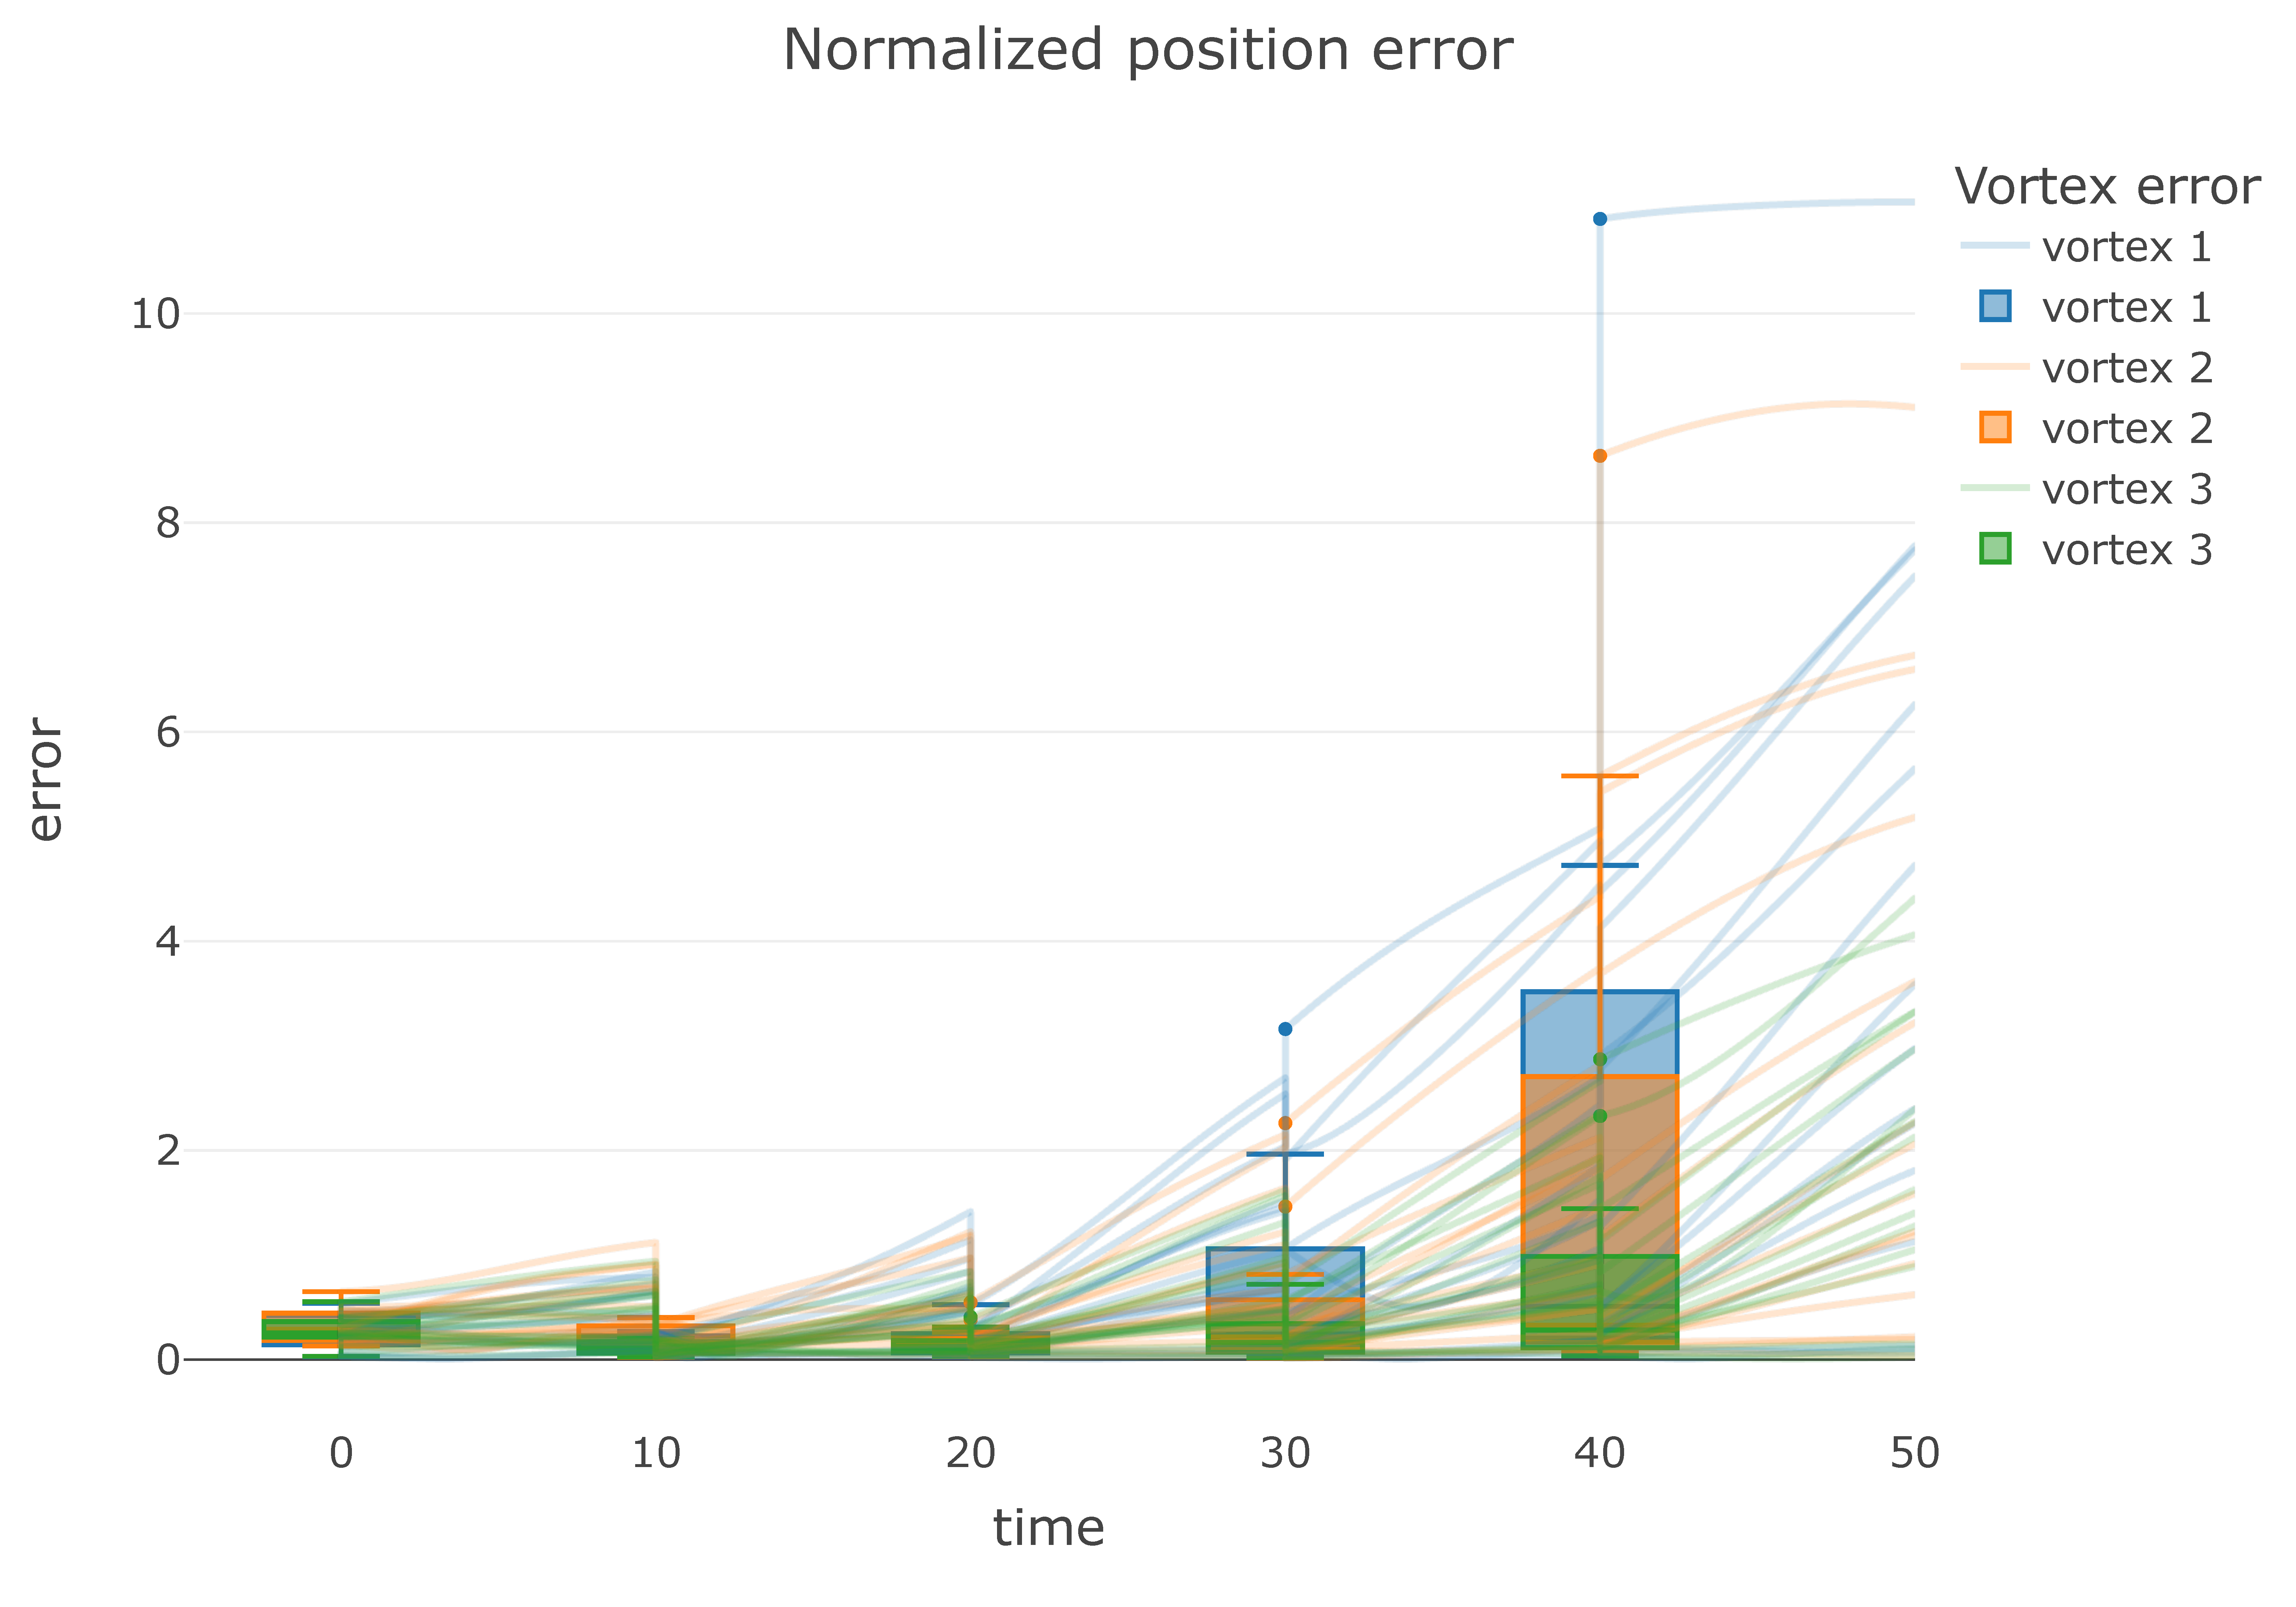
\includegraphics[width=\textwidth]{../../conference/images/part_enkf_error.pdf}
            \end{figure}

            \begin{itemize}
                \item \textbf{pas un cas adéquat} pour appliquer le filtre Part-EnKF
            \end{itemize}
        \end{column}
    \end{columns}
\end{frame}

\begin{frame}{Correction de la position}
    \vspace{-0.5cm}
    \begin{columns}[c]
        \begin{column}{0.45\textwidth}
            \begin{figure}
                \centering
                \caption*{\tiny Alignement du champ du membre un lors de la première étape d'assimilation.}
                \includegraphics<1>[width=\textwidth]{../../conference/images/align_member/align_member_prior.pdf}
                \includegraphics<2>[width=\textwidth]{../../conference/images/align_member/align_member_prior_field.pdf}
                \includegraphics<3->[width=\textwidth]{../../conference/images/align_member/align_member_final.pdf}
            \end{figure}
        \end{column}
        \begin{column}{0.55\textwidth}
            \begin{figure}[c]
                \centering
                \caption*{\tiny Correction du champ de vorticité lors de la première étape d'assimilation.}
                \begin{subfigure}{0.49\textwidth}
                    \centering
                    \includegraphics<1-2>[width=\textwidth]{../../conference/images/vorticity_prior.pdf}
                    \only<1-2>{\caption*{\tiny Avant alignement}}
                    \includegraphics<3>[width=\textwidth]{../../conference/images/vorticity_align.pdf}
                    \only<3>{\caption*{\tiny Après alignement}}
                \end{subfigure}
                \begin{subfigure}{0.49\textwidth}
                    \centering
                    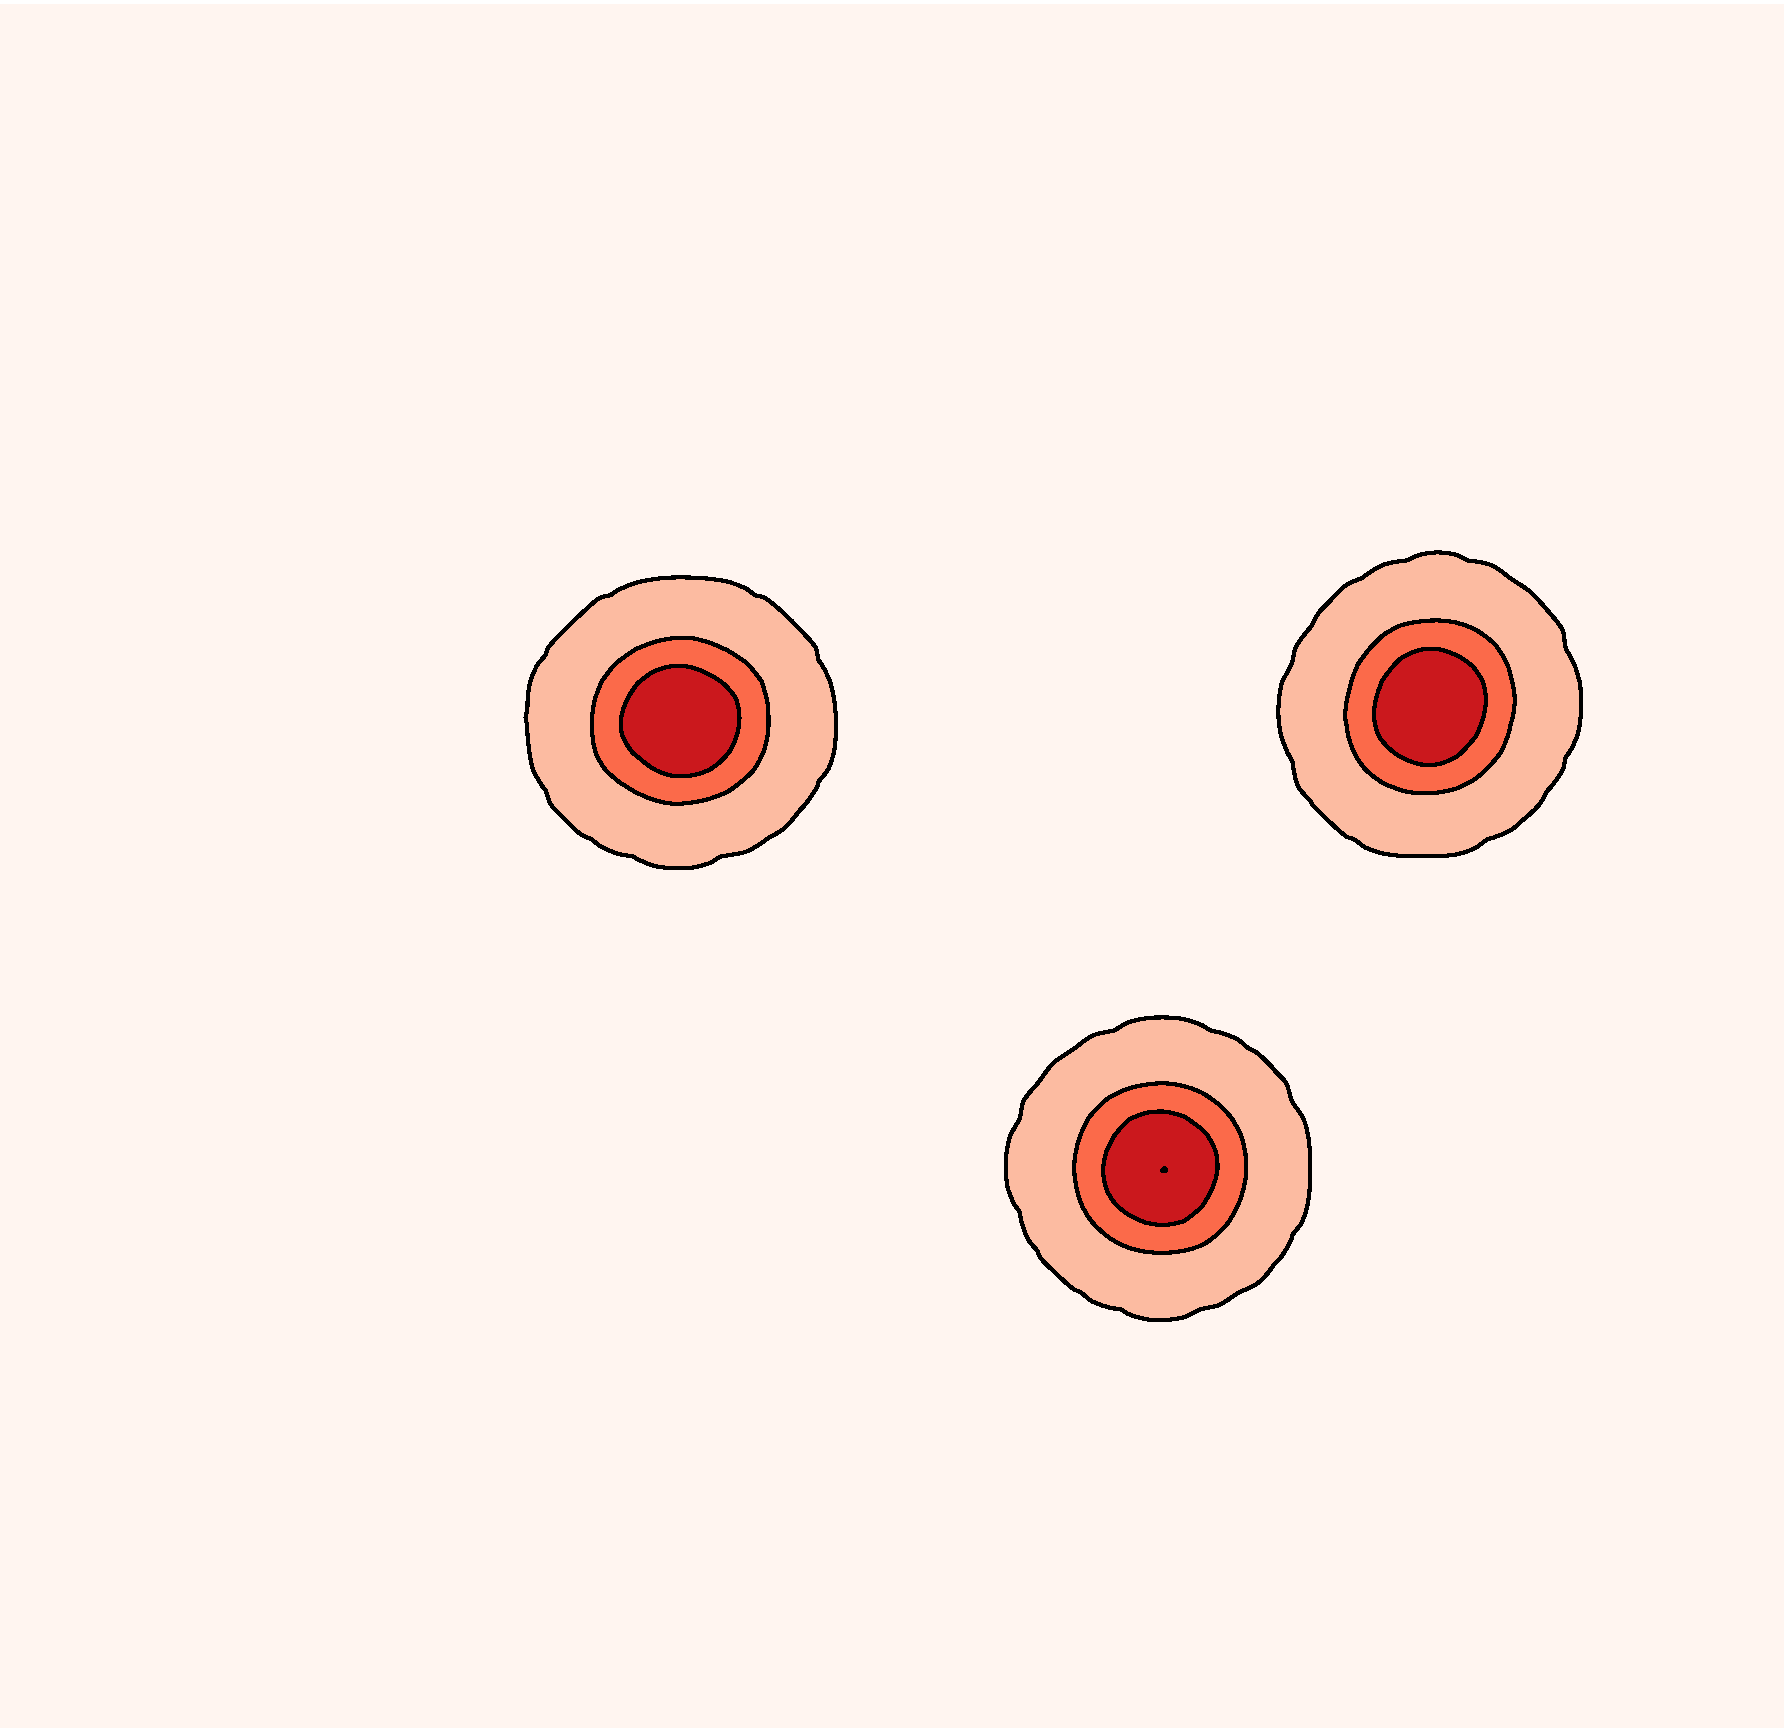
\includegraphics[width=\textwidth]{../../conference/images/vorticity_ref.pdf}
                    \caption*{\tiny Référence}
                \end{subfigure}
            \end{figure}
        \end{column}
    \end{columns}
    \vspace{-0.25cm}
\end{frame}

\begin{frame}{Correction de la position}
    \vspace{-0.5cm}
    \begin{columns}
        \begin{column}{0.5\textwidth}
            \begin{figure}
                \centering
                \animategraphics[loop, autoplay, width=\textwidth]{10}{../../conference/images/vortex_centers_align/vortex_centers_}{0}{36}
                % \caption*{Vortex center trajectories}
            \end{figure}
        \end{column}
        \begin{column}{0.5\textwidth}
            \begin{figure}
                \centering
                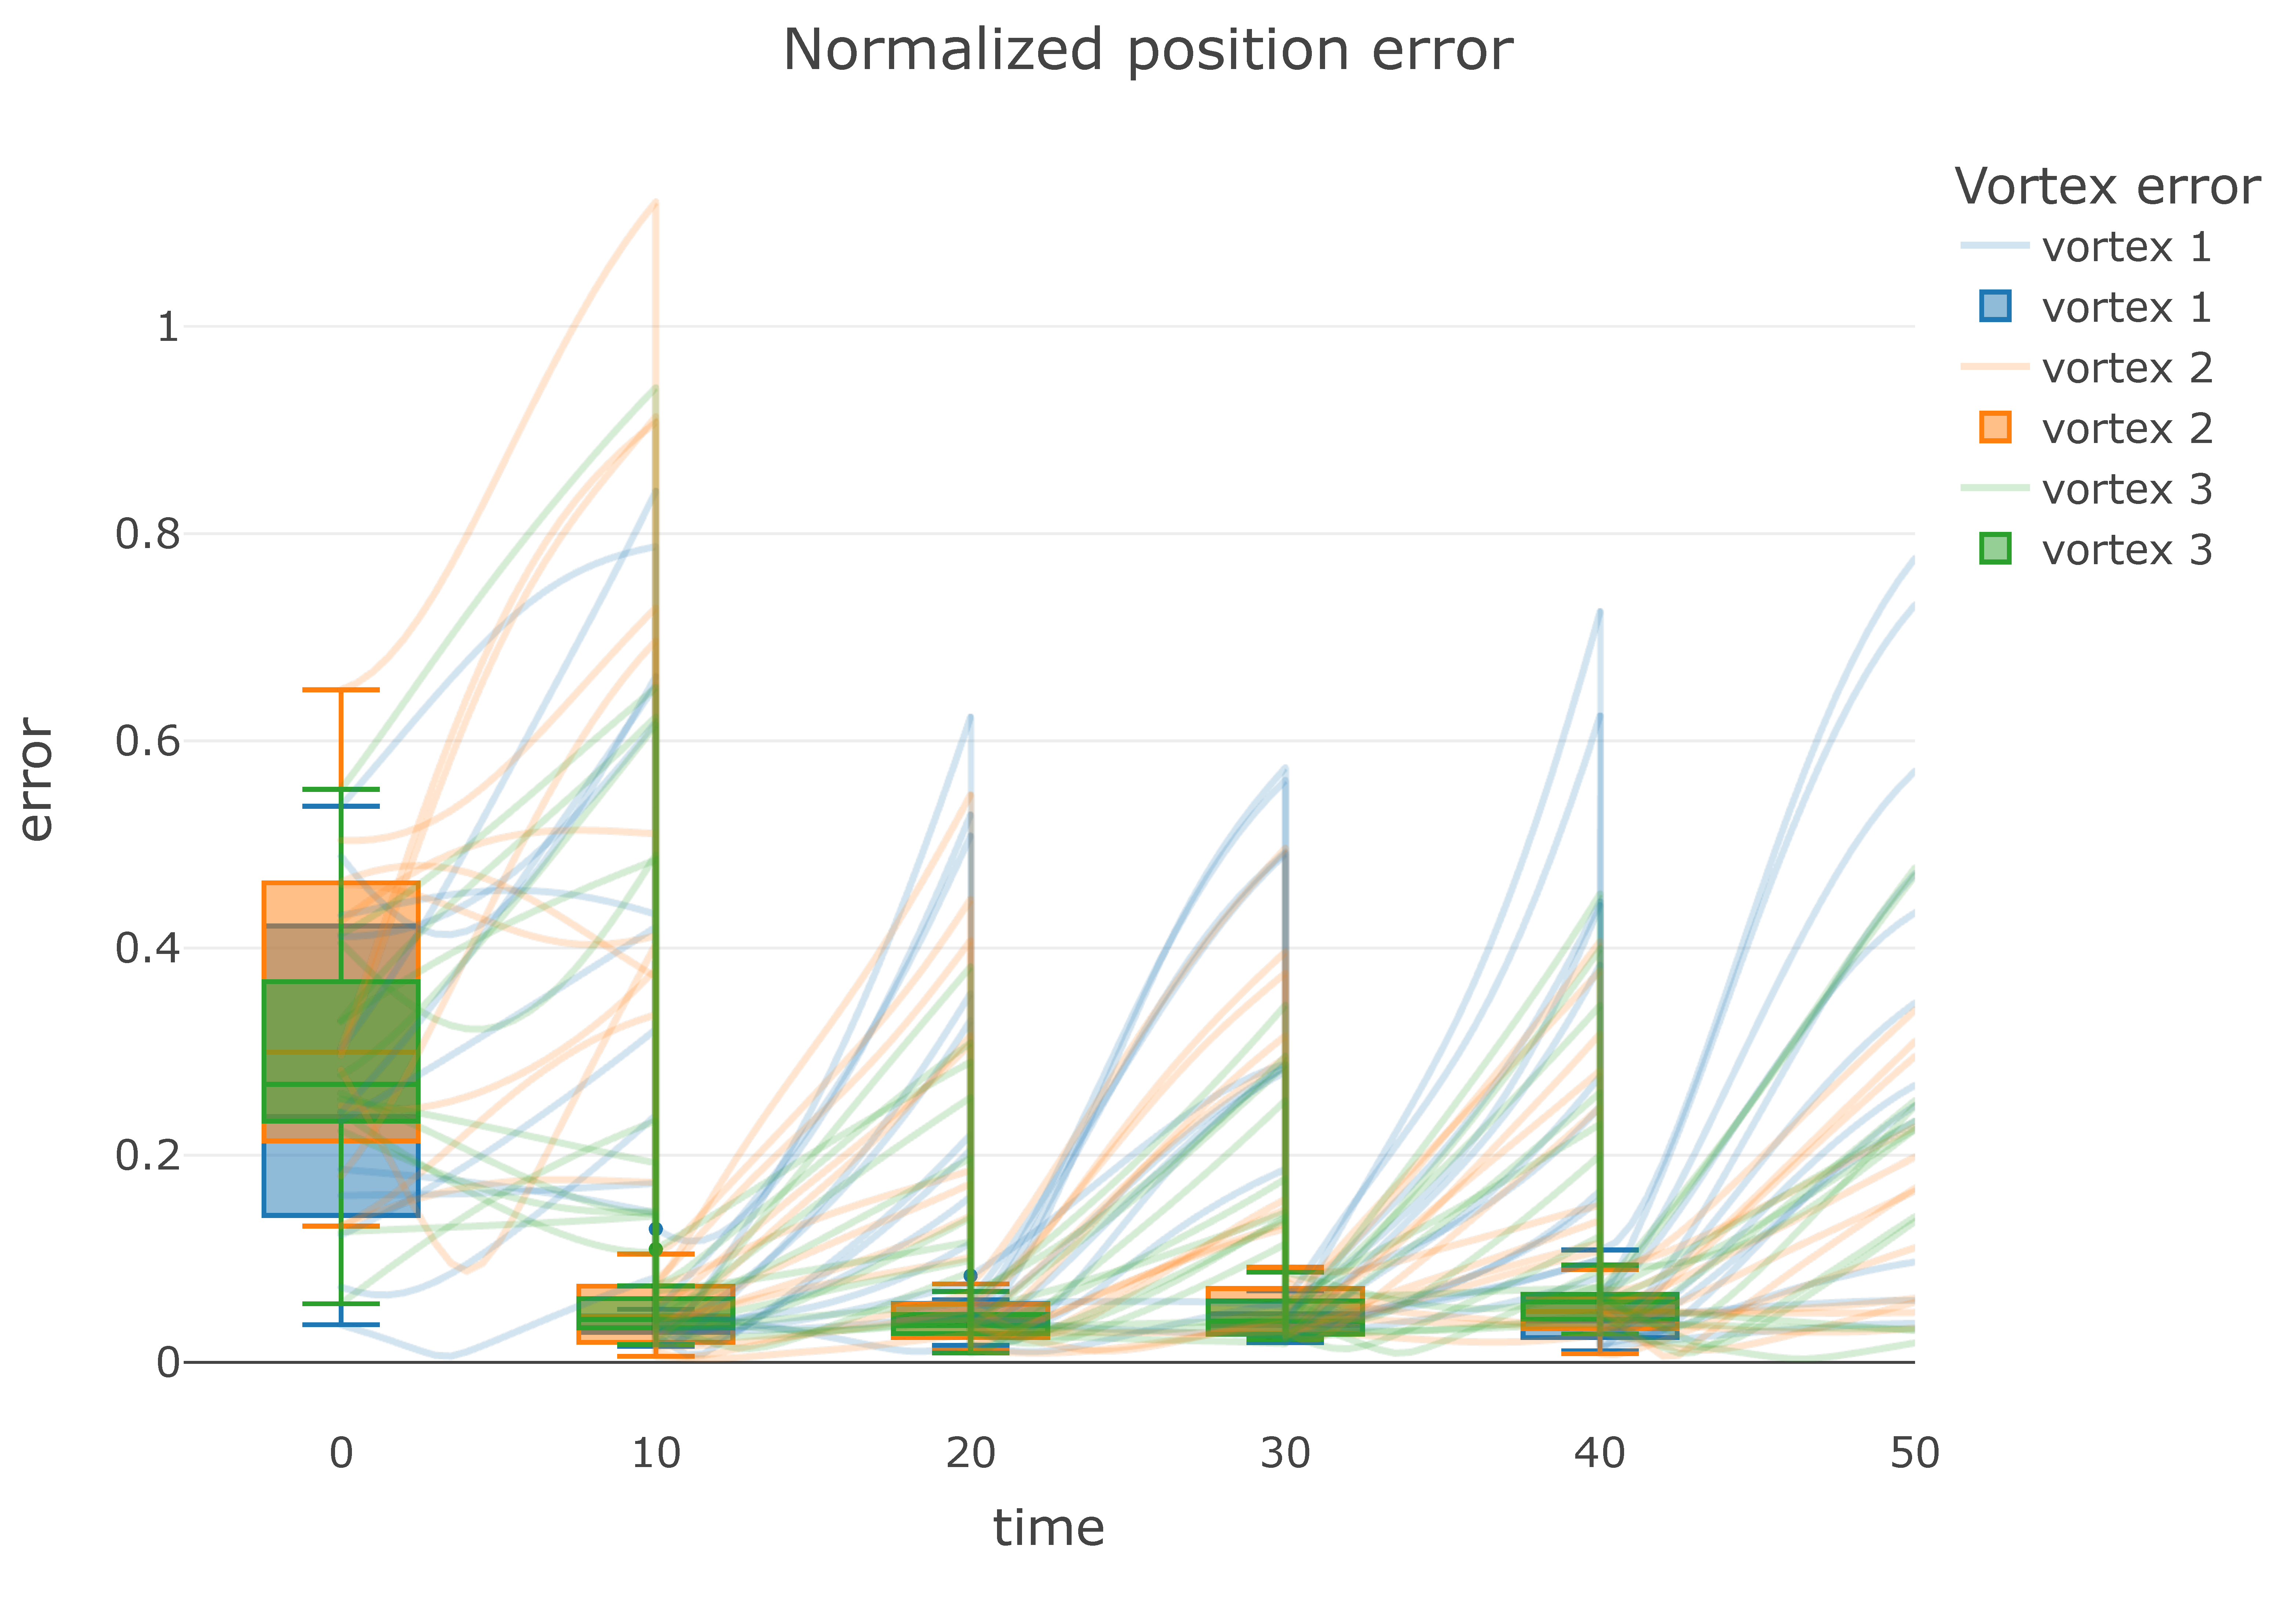
\includegraphics[width=\textwidth]{../../conference/images/align_error.pdf}
                % \caption*{Vortex position error}
            \end{figure}
            \begin{itemize}
                \item Correction de l'erreur de position à chaque assimilation
                \item Mais variabilité à cause de l'incertitude sur les intensités
            \end{itemize}
        \end{column}
    \end{columns}
\end{frame}

\begin{frame}{Correction de la position et de l'intensité}
    \vspace{-0.5cm}
    \begin{columns}
        \begin{column}{0.5\textwidth}
            \begin{figure}
                \centering
                \animategraphics[loop, autoplay, width=\textwidth]{10}{../../conference/images/vortex_centers_part_align/vortex_centers_}{0}{36}
                % \caption*{Vortex center trajectories}
            \end{figure}
        \end{column}
        \begin{column}{0.5\textwidth}
            \begin{figure}
                \centering
                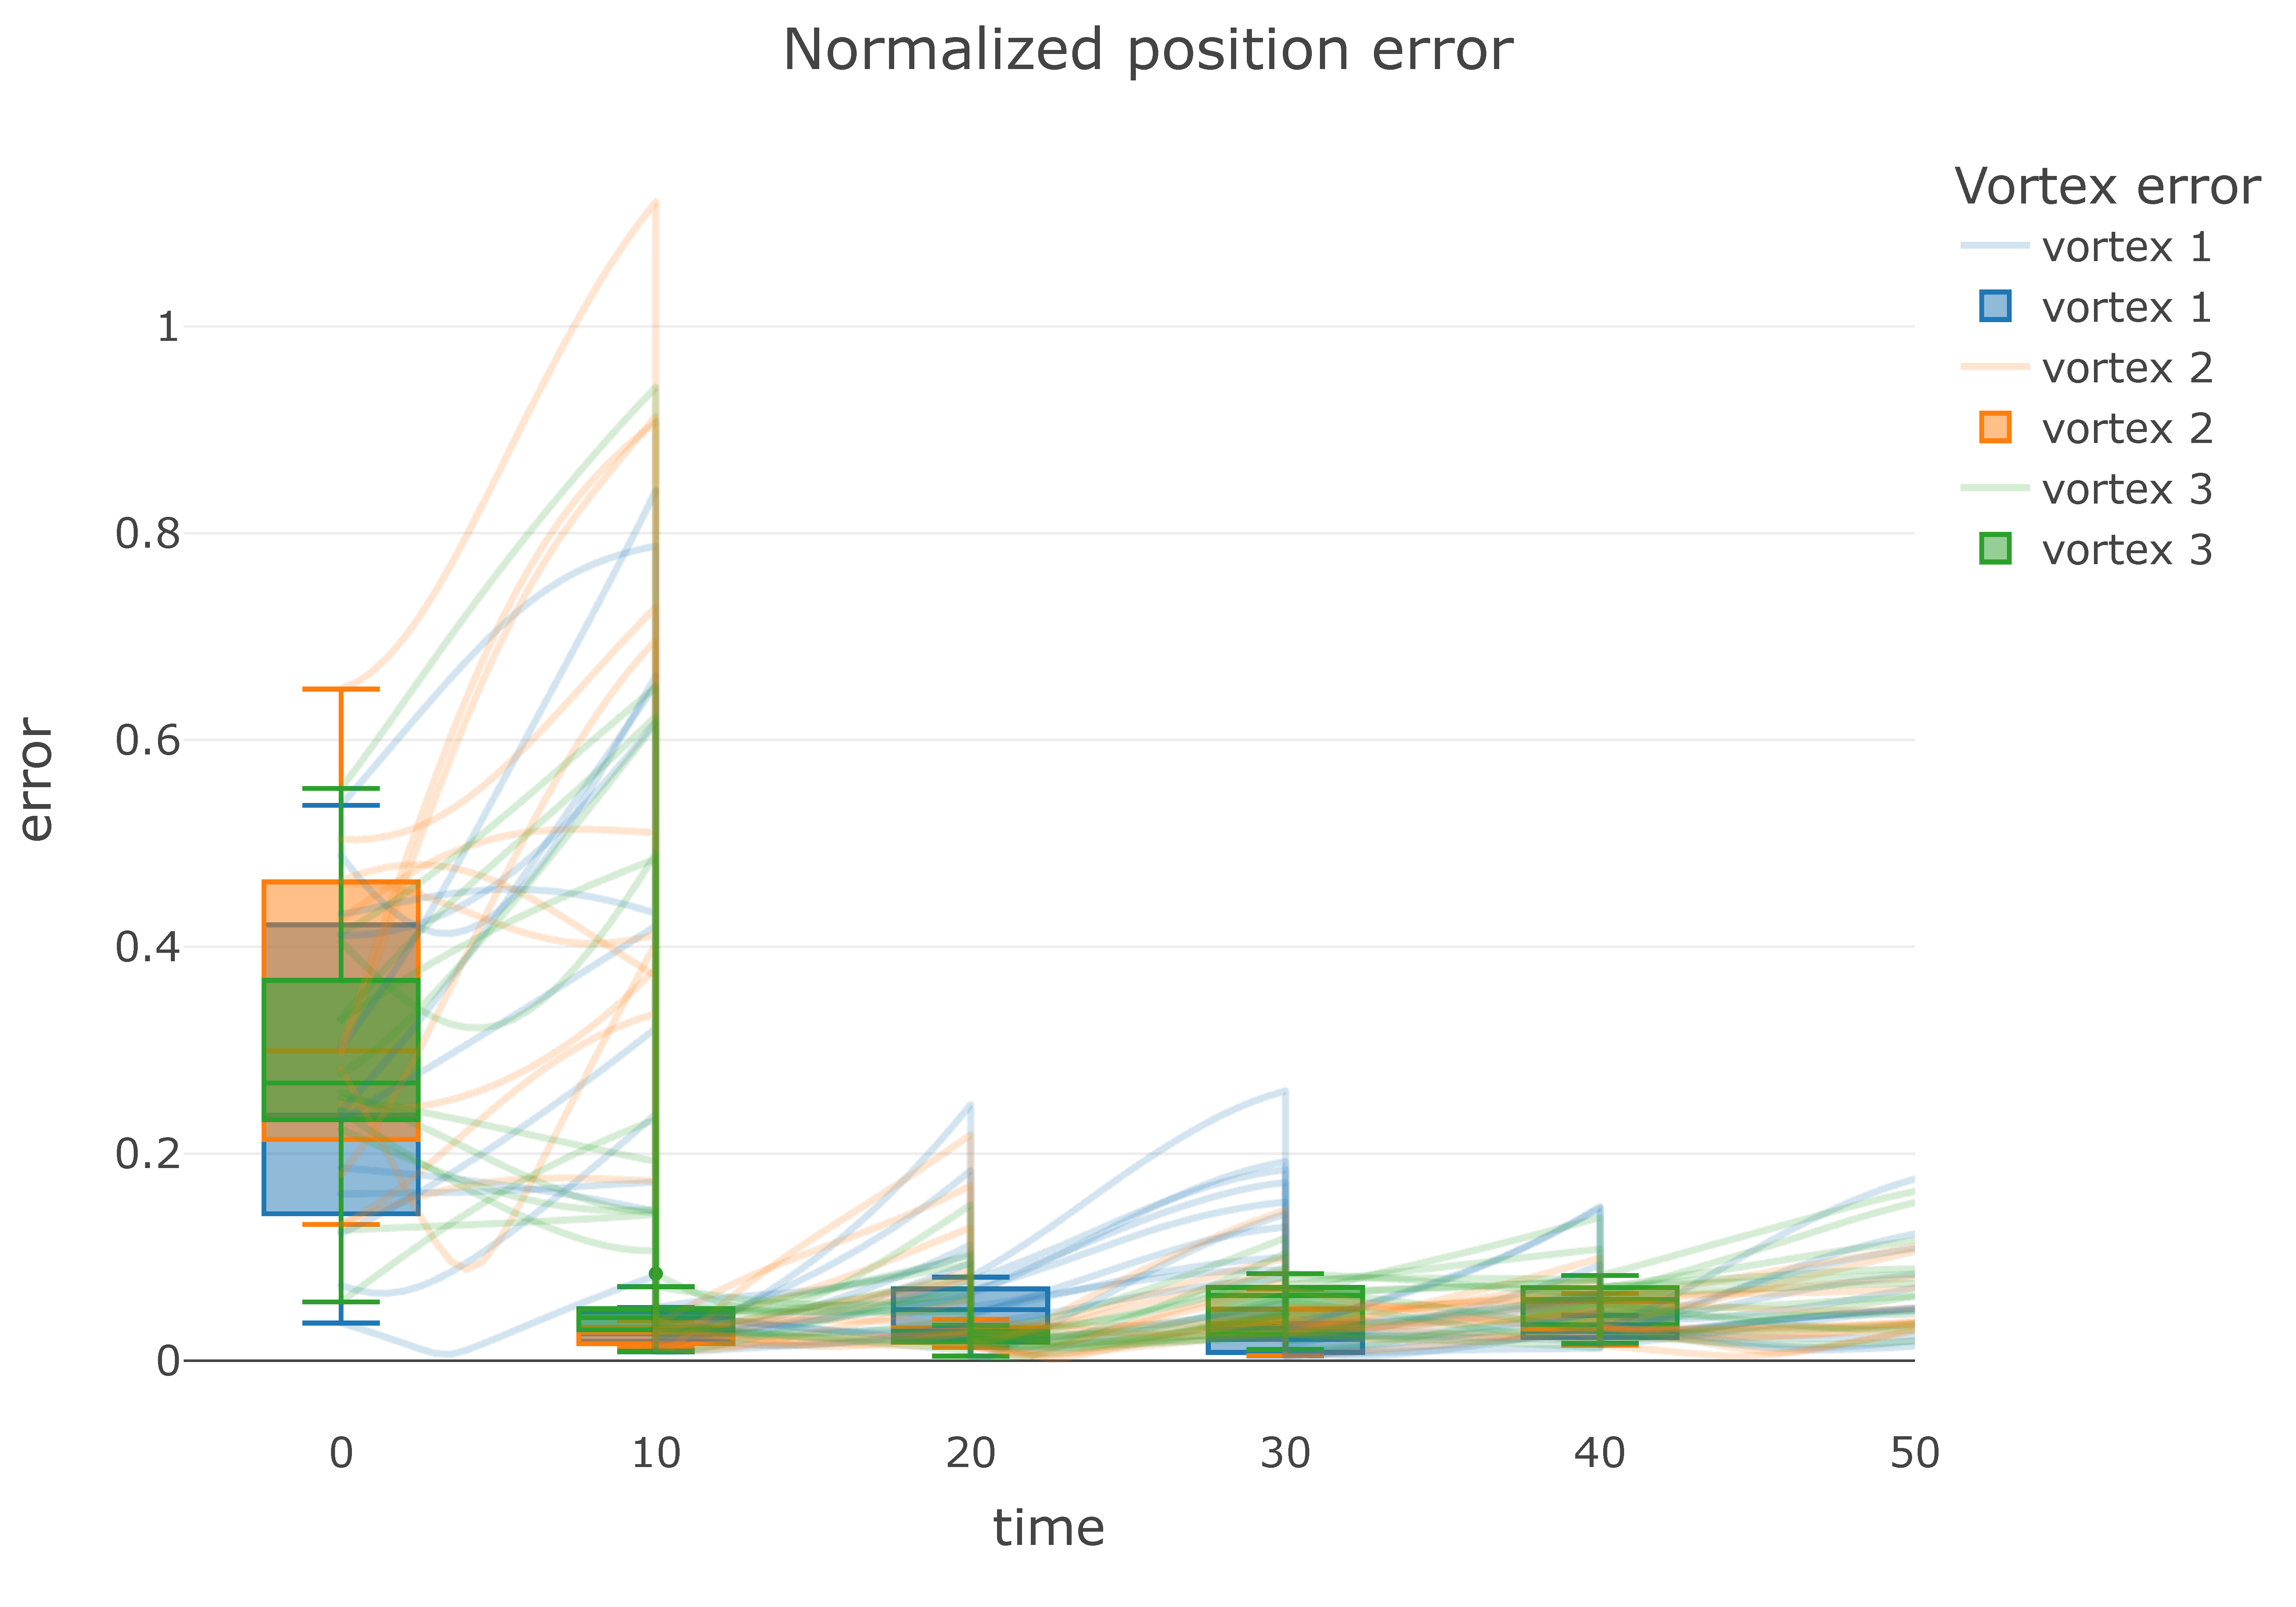
\includegraphics[width=\textwidth]{../../conference/images/align_part_error.pdf}
            \end{figure}

            Correction séquentielle de la \textbf{position} puis de l'\textbf{intensité}
        \end{column}
    \end{columns}
\end{frame}

\transition[2]{Informations générales}{}
\section{Informations générales}

\begin{frame}{Informations générales}
    \small
    \begin{block}{Présentation}
        Présentation à ECCOMAS \\
        Présentation CSI \\
        À venir: Café-Thésard
    \end{block}

    \begin{block}{Formations}
        Finalisation de toutes les formations obligatoires \\
        Pour validation par ED
    \end{block}

    \begin{block}{Jury potentiel}
        \textbf{Rapporteurs}:\\
        - \href{https://scholar.google.fr/citations?user=iM6Mv5MAAAAJ&hl=fr}{Maelle Nodet}: Maitresse de conf, HDR, Université de Versailles St-Quentin \\
        - \href{https://www.irisa.fr/prive/memin/resume-3C.html}{Etienne Mémin}: Full Professor Inria Rennes\\
        \textbf{Evaluateurs}: \\
        \href{https://www-sop.inria.fr/members/Mireille.Bossy}{Mireille Bossy}, \href{https://josselin-garnier.org/}{Josselin Garnier}, \href{https://scholar.google.com/citations?user=DokRauAAAAAJ&hl=fr}{Iraj Maortazavi} + Loïc Giraldi, Olivier L.M.
    \end{block}
\end{frame}

\begin{frame}{Retro-planning}
    \begin{figure}
        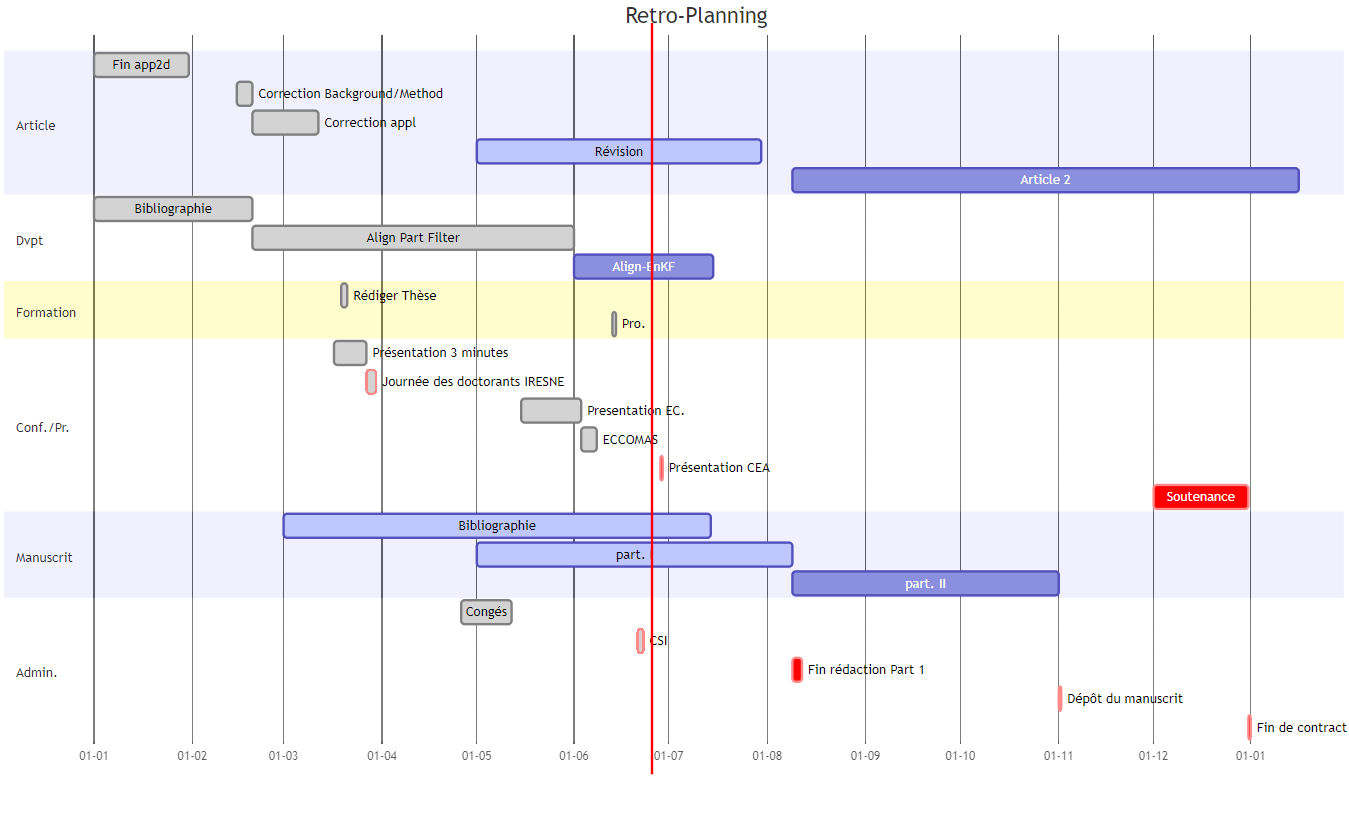
\includegraphics[width=\textwidth]{retro_planning.png}
    \end{figure}
\end{frame}

\begin{frame}[allowframebreaks, noframenumbering]
    \frametitle{References}
    \printbibliography % Print the bibliography
\end{frame}

% \section*{Addendum}
% \begin{frame}{EnKF update}
%   \emph{Be successful with your presentation!}
% \end{frame}

\end{document}